\begin{enumerate}[label=\thechapter.\arabic*,ref=\thechapter.\theenumi]
\numberwithin{equation}{enumi}
\numberwithin{figure}{enumi}
\numberwithin{table}{enumi}

\item Reduce $x-\sqrt{3}y+8=0$ into normal form. Find its perpendicular distance from the origin and angle between perpendicular and the positive x-axis. 
\\
\solution 
		\begin{enumerate}
			\item Optimization Problem
				\\
\label{11/10/3/3/1/conv}
\iffalse
\documentclass[12pt]{article}
\usepackage{graphicx}
\usepackage[none]{hyphenat}
\usepackage{graphicx}
\usepackage{listings}
\usepackage[english]{babel}
\usepackage{graphicx}
\usepackage{caption} 
\usepackage{booktabs}
\usepackage{array}
\usepackage{amssymb} % for \because
\usepackage{amsmath}   % for having text in math mode
\usepackage{extarrows} % for Row operations arrows
\usepackage{listings}
\lstset{
  frame=single,
  breaklines=true
}
\usepackage{hyperref}
  
%Following 2 lines were added to remove the blank page at the beginning
\usepackage{atbegshi}% http://ctan.org/pkg/atbegshi
\AtBeginDocument{\AtBeginShipoutNext{\AtBeginShipoutDiscard}}
\usepackage{gensymb}


%New macro definitions
\newcommand{\mydet}[1]{\ensuremath{\begin{vmatrix}#1\end{vmatrix}}}
\providecommand{\brak}[1]{\ensuremath{\left(#1\right)}}
\providecommand{\sbrak}[1]{\ensuremath{{}\left[#1\right]}}
\providecommand{\norm}[1]{\left\lVert#1\right\rVert}
\providecommand{\abs}[1]{\left\vert#1\right\vert}
\newcommand{\solution}{\noindent \textbf{Solution: }}
\newcommand{\myvec}[1]{\ensuremath{\begin{pmatrix}#1\end{pmatrix}}}
\let\vec\mathbf


\begin{document}

\begin{center}
\title{\textbf{Convex Optimization}}
\date{\vspace{-5ex}} %Not to print date automatically
\maketitle
\end{center}
\setcounter{page}{1}

\section{11$^{th}$ Maths - Chapter 10}
This is Problem-3.1 from Exercise 10.3 
\begin{enumerate}

\solution 
\fi
Let $\vec{O}$ be the point from where we have to find the perpendicular distance and $\vec{P}$ be the foot of the perpendicular. The optimization problem can be expressed as
\begin{align}
	\label{eq:11/10/3/3/1/conv/Eq3}
	  \min_{\vec{x}} \norm{\vec{x}-\vec{O}}^2\\
	 \text{s.t.} \quad \vec{n}^T\vec{x} = c 
\end{align}
where 
\begin{align}
	\vec{n} = \myvec{-1 \\ \sqrt{3}},\,c = 8
\end{align}
The line equation can be expressed as
\begin{align}
	\label{eq:11/10/3/3/1/conv/Eq2}
	\vec{x} = \vec{A}+\lambda\vec{m}
\end{align}
where
\begin{align}
	\label{eq:11/10/3/3/1/conv/Eq1}
	\vec{m} = \myvec{1 \\ \frac{1}{\sqrt{3}}},\,
	\vec{A} = \myvec{-8 \\ 0}
\end{align}
\begin{enumerate}
\item Using the parameric form,
Substituting \eqref{eq:11/10/3/3/1/conv/Eq2} in \eqref{eq:11/10/3/3/1/conv/Eq3}, the optimization problem becomes
\begin{align}
	\min_{\lambda} \norm{ \lambda\vec{m} +\brak{\vec{A}-\vec{O}}}^2\\
	\implies \min_{\lambda}f\brak{\lambda} 	
	= \lambda^2\norm{\vec{m}}^2+ 2\lambda\brak{\vec{A}-\vec{O}}^\top\vec{m}+ + \norm{\vec{A}-\vec{O}}^2  
\label{eq:11/10/3/3/1/conv/Eq4}
\end{align}
$\because$ the coefficient of $\lambda^2> 0$, \eqref{eq:11/10/3/3/1/conv/Eq4} is a convex function.
Thus,
\begin{align}
	f^{\prime\prime}\brak{\lambda} &= 2\norm{\vec{m}}^2 \\ 
	\because f^{\prime\prime}\brak{\lambda} > 0, f^\prime\brak{\lambda_{min}} &= 0, \text{ for } \lambda_{min}
\end{align}
yielding
\begin{align}
	& f^\prime\brak{\lambda_{min}} =  2\lambda_{min}\norm{\vec{m}}^2 + 2\brak{\vec{A}-\vec{O}}^\top\vec{m}  = 0 \\
	\label{eq:11/10/3/3/1/conv/EqMin}
	\lambda_{min} &= -\frac{\brak{\vec{A}-\vec{O}}^\top\vec{m}}{\norm{\vec{m}}^2} 
\end{align}
We choose  
\begin{align}
	\vec{O} &= \myvec{ 0 \\ 0}
\end{align}
Substituting the values of $\vec{A}$, $\vec{O}$ and $\vec{m}$ in equation \eqref{eq:11/10/3/3/1/conv/EqMin}
\begin{align}
	\lambda_{min} &= -\frac{\brak{\myvec{-8 \\ 0 }-\myvec{0 \\ 0}}^\top\myvec{1 \\ \frac{1}{\sqrt{3}}}}{\norm{\myvec{1 \\ \frac{1}{\sqrt{3}}}}^2}\\ 
	&= 6
\end{align}
Substituring this value in equation \eqref{eq:11/10/3/3/1/conv/Eq2}
\begin{align}
	\vec{x}_{min} &= \vec{P} = \myvec{-8 \\ 0}+6\myvec{1 \\ \frac{1}{\sqrt{3}}}  \\
	&= \myvec{-2 \\ 2\sqrt{3}} \\
	OP &= \norm{\vec{P}-\vec{O}}^2 \\ 
	&  = 4
\end{align}
\item Solving using cvxpy, with 
\begin{align}
	&\vec{n} = \myvec{1 \\ -\sqrt{3}} \\
	&\vec{O} = \myvec{0 \\ 0} \\
	&c = -8 \\
	\label{eq:11/10/3/3/1/conv/minval}
	&  \min_{\vec{x}} \norm{\vec{x}-\vec{O}}^2 = 4, 
	 \vec{x}_{min} = \myvec{-2  \\ 3.46 } 
\end{align}
\end{enumerate}
The relevant figures are shown in \ref{fig:11/10/3/3/1/conv/Fig1} and \ref{fig:11/10/3/3/1/conv/Fig2}
\begin{figure}[!h]
	\begin{center}
		\includegraphics[width=\columnwidth]{11/10/3/3/1/conv/figs/problem3.1a.pdf}
	\end{center}
\caption{}
\label{fig:11/10/3/3/1/conv/Fig1}
\end{figure}
\begin{figure}[!h]
	\begin{center}
		\includegraphics[width=\columnwidth]{11/10/3/3/1/conv/figs/problem3.1b.pdf}
	\end{center}
\caption{}
\label{fig:11/10/3/3/1/conv/Fig2}
\end{figure}

\item Gradient Descent
	\\
\label{11/10/3/3/1/grad}
\iffalse
\documentclass[12pt]{article}
\usepackage{graphicx}
\usepackage[none]{hyphenat}
\usepackage{graphicx}
\usepackage{listings}
\usepackage[english]{babel}
\usepackage{graphicx}
\usepackage{caption} 
\usepackage{booktabs}
\usepackage{array}
\usepackage{amsmath}   % for having text in math mode
\usepackage{amssymb} % for \because
\usepackage{extarrows} % for Row operations arrows
\usepackage{listings}
\lstset{
  frame=single,
  breaklines=true
}
\usepackage{hyperref}
  
%Following 2 lines were added to remove the blank page at the beginning
\usepackage{atbegshi}% http://ctan.org/pkg/atbegshi
\AtBeginDocument{\AtBeginShipoutNext{\AtBeginShipoutDiscard}}
\usepackage{gensymb}


%New macro definitions
\newcommand{\mydet}[1]{\ensuremath{\begin{vmatrix}#1\end{vmatrix}}}
\providecommand{\brak}[1]{\ensuremath{\left(#1\right)}}
\providecommand{\sbrak}[1]{\ensuremath{{}\left[#1\right]}}
\providecommand{\norm}[1]{\left\lVert#1\right\rVert}
\providecommand{\cbrak}[1]{\ensuremath{\left\{#1\right\}}}
\providecommand{\abs}[1]{\left\vert#1\right\vert}
\newcommand{\solution}{\noindent \textbf{Solution: }}
\newcommand{\myvec}[1]{\ensuremath{\begin{pmatrix}#1\end{pmatrix}}}
\let\vec\mathbf


\begin{document}

\begin{center}
\title{\textbf{Gradient Descent}}
\date{\vspace{-5ex}} %Not to print date automatically
\maketitle
\end{center}
\setcounter{page}{1}

\section{11$^{th}$ Maths - Chapter 10}
This is Problem-3.1 from Exercise 10.3 
\begin{enumerate}

\solution 
\fi
The given line  can be represented in parametric form as
\begin{align}
	\label{eq:11/10/3/3/1/grad/Eq2}
	\vec{x} = \vec{A}+\lambda\vec{m}
\end{align}
where
\begin{align}
	\vec{A} &= \myvec{-8 \\ 0}\\
	\vec{O} &= \myvec{ 0 \\ 0} \\
	\vec{m} &= \myvec{1 \\ \frac{1}{\sqrt{3}}} \\
\end{align}
 yielding 
\begin{align}
\label{eq:11/10/3/3/1/grad/Eq6}
	f\brak{\lambda} &= \frac{4}{3}\lambda^2-16\lambda+64 \\ 
	f^\prime\brak{\lambda} &= \frac{8}{3}\lambda - 16
\end{align}
Computing $\lambda_{min}$ using Gradient Descent method:
\begin{align}
	\lambda_{n+1} &= \lambda_n - \alpha f^\prime\brak{\lambda_n}\\
	\label{eq:11/10/3/3/1/grad/grad_des}
	\lambda_{n+1} &= \lambda_n\brak{1-\frac{8}{3}\alpha} + 16\alpha
\end{align}
Taking the one-sided $Z$-transform on both sides of \eqref{eq:11/10/3/3/1/grad/grad_des},
\begin{align}
            \label{eq:11/10/3/3/1/grad/Z-trans-eqn}
	    z\Lambda\brak{z} &= \brak{1-\frac{8}{3}\alpha}\Lambda\brak{z} + \frac{16\alpha}{1-z^{-1}} \\
	    \Lambda\brak{z} &= \frac{16\alpha z^{-1}}{\brak{1-z^{-1}}\brak{1-\brak{1-\frac{8}{8}\alpha}z^{-1}}} \\
	    &= 6\brak{ \frac{1}{1-z^{-1}} - \frac{1}{1-\brak{1-\frac{8}{3}\alpha}z^{-1}}} \\
            \label{eq:11/10/3/3/1/grad/lambda-z-trans}
	    &= 6\sum_{k=0}^{\infty}\brak{1-\brak{1-\frac{8}{3}\alpha}^k}z^{-k}
\end{align}
From \eqref{eq:11/10/3/3/1/grad/lambda-z-trans}, the ROC is
\begin{align}
	\abs{z} &> \max\cbrak{1,\abs{1-\frac{8}{3}\alpha}} \\
	\implies -1 & < \abs{1-\frac{8}{3}\alpha} < 1 \\
        \label{eq:11/10/3/3/1/grad/alpha-constr}
        \implies 0 &< \alpha < \frac{3}{4}
\end{align}
Thus, if $\alpha$ satisfies \eqref{eq:11/10/3/3/1/grad/alpha-constr}, then from \eqref{eq:11/10/3/3/1/grad/lambda-z-trans}, 
\begin{align}
	\label{eq:11/10/3/3/1/grad/conv}
        \lim_{n\to\infty}\lambda_n &= 6 
    \end{align}
Choosing
\begin{enumerate}
 \item $\alpha$ = 0.001
 \item precision = 0.0000001
 \item n = 10000000 
 \item $\lambda_0$ = -5 
\end{enumerate}
\begin{align}
	\lambda_{min} &= 6 
\end{align}
Substituting the values of $\vec{A}$, $\vec{m}$ and $\lambda_{min}$ in equation \eqref{eq:11/10/3/3/1/grad/Eq2} 
\begin{align}
	\vec{x}_{min} &= \vec{P} = \myvec{-8 \\ 0}+6\myvec{1 \\ \frac{1}{\sqrt{3}}}  \\
	&= \myvec{-8 \\ 0}+\myvec{6 \\ \frac{6}{\sqrt{3}}} \\
	&= \myvec{-2 \\ 2\sqrt{3}} \\
	OP &= \norm{\vec{P}-\vec{O}}^2 \\ 
	&= \norm{\myvec{-2 \\ 2\sqrt{3}}-\myvec{0 \\ 0}} \\
	&= \sqrt{2^2 + 12} = \sqrt{16} = 4
\end{align}
See Figs. \ref{fig:11/10/3/3/1/grad/Fig1} and \ref{fig:11/10/3/3/1/grad/Fig2}.
\begin{figure}[!h]
	\begin{center}
		\includegraphics[width=\columnwidth]{11/10/3/3/1/grad/figs/problem3.1a.pdf}
	\end{center}
\caption{}
\label{fig:11/10/3/3/1/grad/Fig1}
\end{figure}
\begin{figure}[!h]
	\begin{center}
		\includegraphics[width=\columnwidth]{11/10/3/3/1/grad/figs/problem3.1b.pdf}
	\end{center}
\caption{}
\label{fig:11/10/3/3/1/grad/Fig2}
\end{figure}

			\item Lagrange Multipliers
				\\
\label{11/10/3/3/1/lagmul}
\iffalse
\documentclass[12pt]{article}
\usepackage{graphicx}
\usepackage[none]{hyphenat}
\usepackage{graphicx}
\usepackage{listings}
\usepackage[english]{babel}
\usepackage{graphicx}
\usepackage{caption} 
\usepackage{booktabs}
\usepackage{array}
\usepackage{amssymb} % for \because
\usepackage{amsmath}   % for having text in math mode
\usepackage{extarrows} % for Row operations arrows
\usepackage{listings}
\lstset{
  frame=single,
  breaklines=true
}
\usepackage{hyperref}
  
%Following 2 lines were added to remove the blank page at the beginning
\usepackage{atbegshi}% http://ctan.org/pkg/atbegshi
\AtBeginDocument{\AtBeginShipoutNext{\AtBeginShipoutDiscard}}
\usepackage{gensymb}


%New macro definitions
\newcommand{\mydet}[1]{\ensuremath{\begin{vmatrix}#1\end{vmatrix}}}
\providecommand{\brak}[1]{\ensuremath{\left(#1\right)}}
\providecommand{\sbrak}[1]{\ensuremath{{}\left[#1\right]}}
\providecommand{\norm}[1]{\left\lVert#1\right\rVert}
\providecommand{\abs}[1]{\left\vert#1\right\vert}
\newcommand{\solution}{\noindent \textbf{Solution: }}
\newcommand{\myvec}[1]{\ensuremath{\begin{pmatrix}#1\end{pmatrix}}}
\let\vec\mathbf


\begin{document}

\begin{center}
\title{\textbf{Lagrange Multipliers}}
\date{\vspace{-5ex}} %Not to print date automatically
\maketitle
\end{center}
\setcounter{page}{1}

\section{11$^{th}$ Maths - Chapter 10}
This is Problem-3.1 from Exercise 10.3 
\begin{enumerate}

\solution 

The equation of the given line is 
\begin{align}
	\myvec{1 \\ -\sqrt{3}}^\top\vec{x}+8 &= 0
\end{align}
Let $\vec{O}$ be the point from where we have to find the perpendicular distance. The perpendicular distance will be the minimum distance from $\vec{O}$ to the line. Let $\vec{P}$ be the foot of the perpendicular. 
\fi
		The given  problem can be formulated as 
\begin{align}
	\label{eq:11/10/3/3/1/lagmul/Eq3}
	\min_{\vec{x}} f\brak{\vec{x}} &= \norm{\vec{x}-\vec{O}}^2\\
	\text{s.t.} \quad g\brak{\vec{x}} = \vec{n}^T\vec{x}-c &= 0 
	\label{eq:11/10/3/3/1/lagmul/Eq1}
\end{align}
where
\begin{align}
	\vec{n} = \myvec{1 \\ -\sqrt{3}},\, 
	\vec{O} = \myvec{0 \\ 0},\,
	\text{ and } c = -8
\end{align}
Define
\begin{align}
	H\brak{\vec{x}, \lambda} &= f\brak{\vec{x}} - \lambda g\brak{\vec{x}} 
\end{align}
and we find that 
\begin{align}
	\nabla f\brak{\vec{x}} &= 2\brak{\vec{x}-\vec{O}} \\
        \nabla g\brak{\vec{x}} &= \vec{n}
\end{align}
We have to find $\lambda \in \mathbb{R}$ such that
\begin{align}
	&\nabla H\brak{\vec{x},\lambda} = 0 \\
        \label{eq:11/10/3/3/1/lagmul/Eqlambda}
	&\implies 2\brak{\vec{x}-\vec{O}} - \lambda\vec{n} = 0 \\
        \label{eq:11/10/3/3/1/lagmul/Eqx}
	&\implies \vec{x} = \frac{\lambda}{2}\vec{n} + \vec{O} 
\end{align}
Substituting \eqref{eq:11/10/3/3/1/lagmul/Eqx} in \eqref{eq:11/10/3/3/1/lagmul/Eq1}
\begin{align}
	\vec{n}^\top\brak{\frac{\lambda}{2}\vec{n} + \vec{O}}-c &= 0 \\
	\implies \lambda &= \frac{2\brak{c-\vec{n}^\top\vec{O}}}{\norm{\vec{n}}^2}
\end{align}
Substituting the value of $\lambda$ in \eqref{eq:11/10/3/3/1/lagmul/Eqlambda}, 
\begin{align}
	\vec{x}_{min} &= \vec{P} = \vec{O}+ \frac{\vec{n}\brak{c-\vec{n}^\top\vec{O}}}{\norm{\vec{n}}^2}\\
	&= \myvec{0 \\0}+ \frac{\myvec{1 \\ -\sqrt{3}}\brak{-8-\myvec{1 & -\sqrt{3}}\myvec{0 \\0}}}{4} \\
	&= \myvec{-2 \\ 2\sqrt{3}} \\
	OP &= \norm{\vec{P}-\vec{O}}^2 \\ 
	&= \norm{\myvec{-2 \\ 2\sqrt{3}}-\myvec{0 \\ 0}} \\
	&=  4
\end{align}	
The relevant figure is shown in \ref{fig:11/10/3/3/1/lagmul/Fig1}
\begin{figure}[!h]
	\begin{center}
		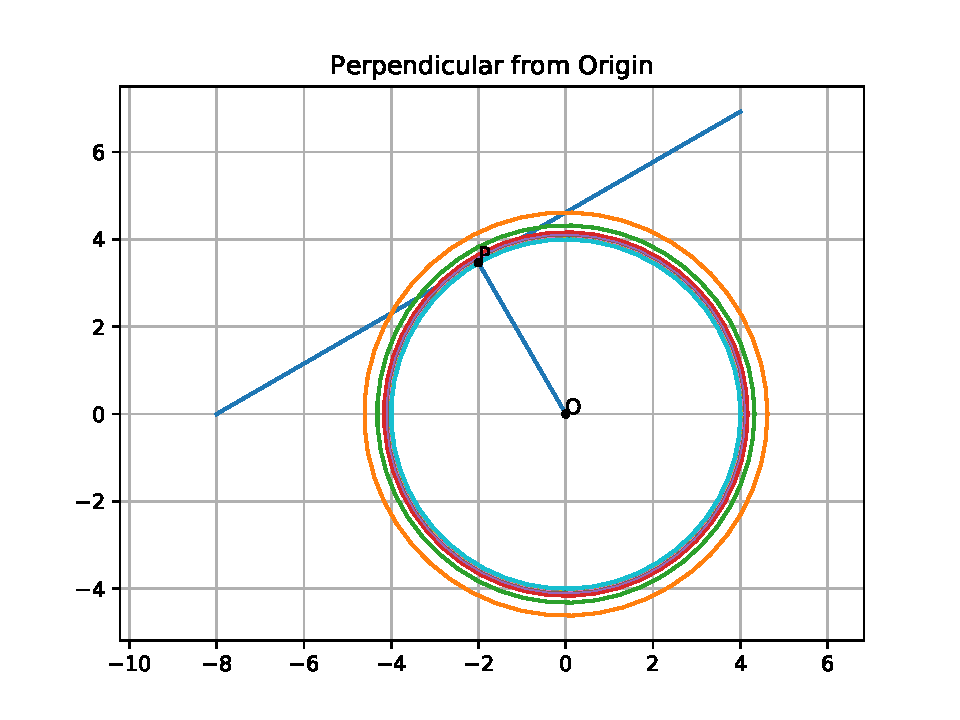
\includegraphics[width=\columnwidth]{11/10/3/3/1/lagmul/figs/problem3.1.pdf}
	\end{center}
\caption{}
\label{fig:11/10/3/3/1/lagmul/Fig1}
\end{figure}

		\end{enumerate}
		%
\item Reduce the equation $y-2=0$ into normal form. Find the perpendicular distances from the origin and angle between perpendicular and the positive x-axis.
\\
\solution 
		\begin{enumerate}
			\item Optimization Problem
				\\
\label{11/10/3/3/2/conv}
\iffalse
\documentclass[12pt]{article}
\usepackage{graphicx}
\usepackage{amsmath}
\usepackage{mathtools}
\usepackage{gensymb}
\usepackage{tabularx}
\usepackage{array}
\usepackage[latin1]{inputenc}
\usepackage{fullpage}
\usepackage{color}
\usepackage{array}
\usepackage{longtable}
\usepackage{calc}
\usepackage{multirow}
\usepackage{hhline}
\usepackage{ifthen}
\usepackage{lscape}
\usepackage{float}
\usepackage{amssymb}

\newcommand{\mydet}[1]{\ensuremath{\begin{vmatrix}#1\end{vmatrix}}}
\providecommand{\brak}[1]{\ensuremath{\left(#1\right)}}
\providecommand{\norm}[1]{\left\lVert#1\right\rVert}
\providecommand{\abs}[1]{\left\vert#1\right\vert}
\newcommand{\solution}{\noindent \textbf{Solution: }}
\newcommand{\myvec}[1]{\ensuremath{\begin{pmatrix}#1\end{pmatrix}}}
\let\vec\mathbf

\def\inputGnumericTable{}

\begin{document}
\begin{center}
\textbf\large{OPTIMIZATION}

\end{center}
\section*{Excercise 10.3}


\solution
\fi
The given equation can be written as
\begin{align}
	\label{eq:11/10/3/3/2/conv/eq1}
	\myvec{0&1}\vec{x} &= 2\\
\implies 	\vec{n} &= \myvec{0\\1},\,
	\vec{m} = \myvec{1\\0}
\end{align}
Equation \eqref{eq:11/10/3/3/2/conv/eq1} can be represented in parametric form as
\begin{align}
	\label{eq:11/10/3/3/2/conv/eq2}
	\vec{x} = \vec{A}+\lambda\vec{m}
\end{align}
where
\begin{align}
	\vec{A} &= \myvec{2\\2}.
	\label{eq:11/10/3/3/2/conv/line}
\end{align}
Let $\vec{O}$ be the origin. The perpendicular distance will be the minimum distance from $\vec{O}$ to the line. Let $\vec{P}$ be the foot of perpendicular. This problem can be formulated as an optimization problem as 
\begin{align}
	d &=  \min_{\vec{x}}\norm{\vec{x}-\vec{O}}^2\\
	&=\min_{\lambda}\norm{\vec{A}+\lambda\vec{m}-\vec{O}}^2\\
	&= f\brak{\lambda} = \norm{\vec{m}}^2\lambda^2+2\vec{A}^\top\vec{m}+\norm{\vec{A}}^2
	\label{eq:11/10/3/3/2/conv/eq3}
	\\
	&= \lambda^2+4\lambda+8
\end{align}
$\because$ the coefficient of $\lambda^2>0$, \eqref{eq:11/10/3/3/2/conv/eq3} is convex. 
\begin{align}
	\label{eq:11/10/3/3/2/conv/eq4}
	f^\prime\brak{\lambda} = 2\norm{\vec{m}}^2\lambda+\brak{\vec{A}^\top\vec{m}+\vec{m}^\top\vec{A}}
\end{align}
\begin{enumerate}
\item Computing $\lambda_{min}$ using Derivative method
\begin{align}
	f^{\prime\prime}\brak{\lambda} &= 2\\
	\because f^{\prime\prime}\brak{\lambda}>0,&f^{\prime}\brak{\lambda_{min}}=0, \text{ for } \lambda_{min}\\
	f^{\prime}\brak{\lambda_{min}} &= 2\norm{\vec{m}}^2\lambda_{min}+\brak{\vec{A}^\top\vec{m}+\vec{m}^\top\vec{A}}\\
	\therefore \lambda_{min} &= -\frac{\brak{\vec{A}^\top\vec{m}+\vec{m}^\top\vec{A}}}{2\norm{\vec{m}}^2} = -2
\end{align}
Thus, 
\begin{align}
	\vec{x}_{min} &= \vec{P} = \myvec{2\\2}+\brak{-2}\myvec{1\\0}\\
	&= \myvec{0\\2}\\
	OP &= \norm{\vec{P}-\vec{O}}\\
	&= \norm{\myvec{0\\2}-\myvec{0\\0}}\\
	&= 2
\end{align}
\item Solving using cvxpy, with
\begin{align}
	\vec{n} &= \myvec{0\\1}\\
	\vec{O} &= \myvec{0\\0}\\
	c &= 2\\
	&\min_{\vec{x}}\norm{\vec{x}-\vec{O}}^2 = 2, \vec{x}_{min} = \myvec{0\\2}
\end{align}
\end{enumerate}
See Figs. \ref{fig:11/10/3/3/2/conv/Fig1} and \ref{fig:11/10/3/3/2/conv/Fig2}.
\begin{figure}[!h]
	\begin{center} 
	    \includegraphics[width=\columnwidth]{11/10/3/3/2/conv/figs/opt1}
	\end{center}
\caption{}
\label{fig:11/10/3/3/2/conv/Fig1}
\end{figure}
\begin{figure}[!h]
	\begin{center} 
	    \includegraphics[width=\columnwidth]{11/10/3/3/2/conv/figs/opt2}
	\end{center}
\caption{}
\label{fig:11/10/3/3/2/conv/Fig2}
\end{figure}

\item Gradient Descent
	\\
\label{11/10/3/3/2/grad}
\iffalse

\documentclass[12pt]{article}
\usepackage{graphicx}
\usepackage{amsmath}
\usepackage{mathtools}
\usepackage{gensymb}
\usepackage{tabularx}
\usepackage{array}
\usepackage[latin1]{inputenc}
\usepackage{fullpage}
\usepackage{color}
\usepackage{array}
\usepackage{longtable}
\usepackage{calc}
\usepackage{multirow}
\usepackage{hhline}
\usepackage{ifthen}
\usepackage{lscape}
\usepackage{float}
\usepackage{amssymb}

\newcommand{\mydet}[1]{\ensuremath{\begin{vmatrix}#1\end{vmatrix}}}
\providecommand{\brak}[1]{\ensuremath{\left(#1\right)}}
\providecommand{\cbrak}[1]{\ensuremath{\left\{#1\right\}}}
\providecommand{\norm}[1]{\left\lVert#1\right\rVert}
\providecommand{\abs}[1]{\left\vert#1\right\vert}
\newcommand{\solution}{\noindent \textbf{Solution: }}
\newcommand{\myvec}[1]{\ensuremath{\begin{pmatrix}#1\end{pmatrix}}}
\let\vec\mathbf

\def\inputGnumericTable{}

\begin{document}
\begin{center}
\textbf\large{OPTIMIZATION}

\end{center}
\section*{Excercise 10.3}


\solution
\fi
The given equation can be represented in parametric form as
\begin{align}
	\label{eq:11/10/3/3/2/grad/eq2}
	\vec{x} = \vec{A}+\lambda\vec{m}
\end{align}
where
\begin{align}
	\vec{A} = \myvec{2\\2}, \vec{m} = \myvec{1\\0}
	\label{eq:11/10/3/3/2/grad/line}
\end{align}
Let $\vec{O}$ be the origin. The perpendicular distance will be the minimum distance from $\vec{O}$ to the line. Let $\vec{P}$ be the foot of perpendicular. This problem can be formulated as an optimization problem as follows:
\begin{align}
	& \min_{\vec{x}}\norm{\vec{x}-\vec{O}}^2\\
	& \implies \min_{\lambda}\norm{\vec{A}+\lambda\vec{m}-\vec{O}}^2\\
	& \implies \min_{\lambda}\norm{\vec{A}+\lambda\vec{m}}^2\\
	\implies f\brak{\lambda} &= \norm{\vec{A+\lambda\vec{m}}}^2\\
	&= \brak{\vec{A}+\lambda\vec{m}}^\top\brak{\vec{A}+\lambda\vec{m}}\\
	&= \norm{\vec{A}}^2+\vec{A}^\top\brak{\lambda\vec{m}}+\brak{\lambda\vec{m}}^\top\vec{A}+\brak{\lambda\vec{m}}^\top\brak{\lambda\vec{m}}\\
	&= \norm{\vec{A}}^2+\lambda\vec{A}^\top\vec{m}+\lambda\vec{m}^\top\vec{A}+\lambda^2\norm{\vec{m}}^2\\
	&= \norm{\vec{m}}^2\lambda^2+\brak{\vec{A}^\top\vec{m}+\vec{m}^\top\vec{A}}\lambda+\norm{\vec{A}}^2\\
	\label{eq:11/10/3/3/2/grad/eq3}
	&= \lambda^2+4\lambda+8
\end{align}
$\because$ the coefficient of $\lambda^2>0$, equation \eqref{eq:11/10/3/3/2/grad/eq3} is a convex function
\begin{align}
	\label{eq:11/10/3/3/2/grad/eq4}
	f^\prime\brak{\lambda} = 2\lambda+4
\end{align}
Computing $\lambda_{min}$ using Gradient Descent method:
\begin{align}
	\lambda_{n+1} &= \lambda_n - \alpha\nabla f\brak{\lambda_n}\\
	\label{eq:11/10/3/3/2/grad/eq5}
	\lambda_{n+1} &= \brak{1-2\alpha}\lambda_{n} - 4\alpha
\end{align}
Taking one-sided Z-transform on both sides of \eqref{eq:11/10/3/3/2/grad/eq5},
\begin{align}
	z\Lambda\brak{z} &= \brak{1-2\alpha}\Lambda\brak{z} - \frac{4\alpha}{1-z^{-1}}\\
	\Lambda\brak{z} &= -\frac{4\alpha z^{-1}}{\brak{1-\brak{1-2\alpha}z^{-1}}\brak{1-z^{-1}}}\\
	&= 2\brak{\frac{1}{\brak{1-\brak{1-2\alpha}z^{-1}}}-\frac{1}{1-z^{-1}}}\\
	\label{eq:11/10/3/3/2/grad/eq6}
	&= 2\sum_{k=0}^{\infty}\brak{\brak{1-2\alpha}^{k}-1}z^{-k}
\end{align}
from \eqref{eq:11/10/3/3/2/grad/eq6}, the ROC is
\begin{align}
	\abs{z}>\max\cbrak{{1,\abs{1-2\alpha}}}\\
	\implies 0<\abs{1-2\alpha}<1\\
	\label{eq:11/10/3/3/2/grad/eq7}
	\implies 0<\alpha<\frac{1}{2}
\end{align}
Thus, if $\alpha$ satisfies \eqref{eq:11/10/3/3/2/grad/eq7}, then from \eqref{eq:11/10/3/3/2/grad/eq6}
\begin{align}
	\lim_{n\to\infty} \lambda_{n} = -2
\end{align}
Choosing
\begin{enumerate}
\item $\alpha$ = 0.001
\item precision = 0.0000001
\item n = 10000000
\item $\lambda_0$ = 4
\begin{align}
	\lambda_{min} = -2
\end{align}
\end{enumerate}
\begin{align}
	\vec{x}_{min} &= \vec{P} = \myvec{2\\2}+\brak{-2}\myvec{1\\0}\\
	&= \myvec{0\\2}\\
	OP &= \norm{\vec{P}-\vec{O}}\\
	&= \norm{\myvec{0\\2}-\myvec{0\\0}}\\
	&= 2
\end{align}
See figure \ref{fig:11/10/3/3/2/grad/Fig1} and figure \ref{fig:11/10/3/3/2/grad/Fig2}
\begin{figure}[!h]
	\begin{center} 
	    \includegraphics[width=\columnwidth]{11/10/3/3/2/grad/figs/opt1}
	\end{center}
\caption{}
\label{fig:11/10/3/3/2/grad/Fig1}
\end{figure}
\begin{figure}[!h]
	\begin{center} 
	    \includegraphics[width=\columnwidth]{11/10/3/3/2/grad/figs/opt2}
	\end{center}
\caption{}
\label{fig:11/10/3/3/2/grad/Fig2}
\end{figure}

			\item Lagrange Multipliers
				\\
\label{11/10/3/3/2/lagmul}
\iffalse
\documentclass[12pt]{article}
\usepackage{graphicx}
\usepackage{amsmath}
\usepackage{mathtools}
\usepackage{gensymb}
\usepackage{tabularx}
\usepackage{array}
\usepackage[latin1]{inputenc}
\usepackage{fullpage}
\usepackage{color}
\usepackage{array}
\usepackage{longtable}
\usepackage{calc}
\usepackage{multirow}
\usepackage{hhline}
\usepackage{ifthen}
\usepackage{lscape}
\usepackage{float}
\usepackage{amssymb}

\newcommand{\mydet}[1]{\ensuremath{\begin{vmatrix}#1\end{vmatrix}}}
\providecommand{\brak}[1]{\ensuremath{\left(#1\right)}}
\providecommand{\cbrak}[1]{\ensuremath{\left\{#1\right\}}}
\providecommand{\norm}[1]{\left\lVert#1\right\rVert}
\providecommand{\abs}[1]{\left\vert#1\right\vert}
\newcommand{\solution}{\noindent \textbf{Solution: }}
\newcommand{\myvec}[1]{\ensuremath{\begin{pmatrix}#1\end{pmatrix}}}
\let\vec\mathbf

\def\inputGnumericTable{}

\begin{document}
\begin{center}
\textbf\large{OPTIMIZATION}

\end{center}
\section*{Excercise 10.3}

Q.3.2 
\solution
The given equation can be written as
\begin{align}
	\label{eq:11/10/3/3/2/lagmul/eq1}
	\myvec{0&1}\vec{x} &= 2
\end{align}
Let $\vec{O}$ be the point from where we have to find the perpendicular distance. The perpendicular distance will be the minimum distance from $\vec{O}$ to theline. Let $\vec{P}$ be the foot of perpendicular. 
\fi
The given problem can be formulated as 
\begin{align}
	\min_{\vec{x}}f\brak{\vec{x}} &= \norm{\vec{x}-\vec{O}}^2\\
	\text{s.t. } g\brak{\vec{x}} &= \vec{n}^\top\vec{x}-c=0
	\label{eq:11/10/3/3/2/lagmul/eq1}
\end{align}
where
\begin{align}
	\vec{n} = \myvec{0\\1},\,
	\vec{O} = \myvec{0\\0},
	c = 2
\end{align}
Define
\begin{align}
	H\brak{\vec{x},\lambda} = f\brak{\vec{x}} - \lambda g\brak{\vec{x}}
\end{align}
Since
\begin{align}
	\nabla f\brak{\vec{x}} &= 2\brak{\vec{x}-\vec{O}}\\
	\nabla g\brak{\vec{x}} &= \vec{n}
\end{align}
We have to find $\lambda \in \mathbb{R}$ such that
\begin{align}
	\nabla H\brak{\vec{x},\lambda} &= 0\\
	\label{eq:11/10/3/3/2/lagmul/eq2}
	\implies 2\brak{\vec{x}-\vec{O}}-\lambda\vec{n} &= 0\\
	\label{eq:11/10/3/3/2/lagmul/eq3}
	\implies \vec{x} = \frac{\lambda}{2}\vec{n}+\vec{O}
\end{align}
Substituting \eqref{eq:11/10/3/3/2/lagmul/eq3} in \eqref{eq:11/10/3/3/2/lagmul/eq1}
\begin{align}
	\vec{n}^\top\brak{\frac{\lambda}{2}\vec{n}+\vec{O}} - c &= 0\\
	\implies \lambda = \frac{2\brak{c-\vec{n}^\top\vec{O}}}{\norm{\vec{n}}^2} &= 4 > 0
\end{align}
Substituting the value of $\lambda$ in \eqref{eq:11/10/3/3/2/lagmul/eq3},
\begin{align}
	\vec{x}_{min} &=  \vec{O}+\frac{\vec{n}\brak{c-\vec{n}^\top\vec{O}}}{\norm{\vec{n}}^2}
	\\
	&= \myvec{0\\0}+ \frac{\myvec{0\\1}\brak{2-\myvec{0&1}\myvec{0\\0}}}{1}
	= \myvec{0\\2}\\
	\implies OP &= \norm{\vec{P}-\vec{O}}^2
	= 2
\end{align}
See Fig. \ref{fig:11/10/3/3/2/lagmul/Fig1}
\begin{figure}[!h]
	\begin{center} 
	    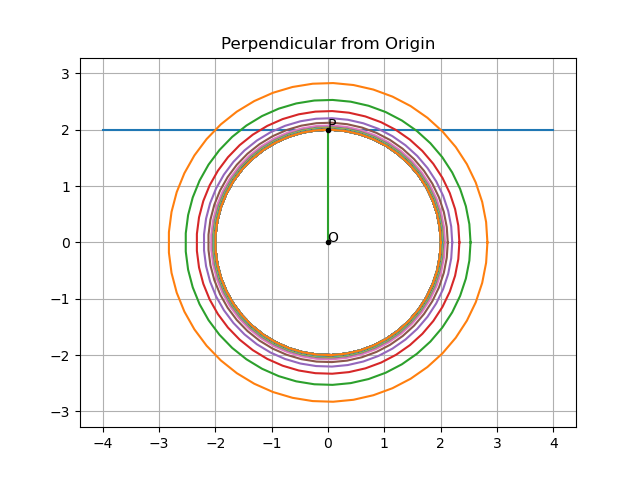
\includegraphics[width=\columnwidth]{11/10/3/3/2/lagmul/figs/opt3}
	\end{center}
\caption{}
\label{fig:11/10/3/3/2/lagmul/Fig1}
\end{figure}

		\end{enumerate}
  \item Find the coordinates of the foot of perpendicular from the point 
    \begin{align}
        \vec{P} = \myvec{-1\\3}
        \label{eq:11/10/3/14/lagmul/P-def}
    \end{align}
    to the line 
    \begin{align}
        \myvec{3&-4}\vec{x} = 16
        \label{eq:11/10/3/14/lagmul/line}
    \end{align}
	  \\
		\solution
		\begin{enumerate}
			\item Optimization Problem
				\\
\label{11/10/3/14/conv}
\iffalse
\documentclass[journal,12pt,twocolumn]{IEEEtran}
\usepackage{setspace}
\usepackage{gensymb}
\singlespacing
\usepackage[cmex10]{amsmath}
\usepackage{amsthm}
\usepackage{mathrsfs}
\usepackage{txfonts}
\usepackage{stfloats}
\usepackage{bm}
\usepackage{cite}
\usepackage{cases}
\usepackage{subfig}
\usepackage{longtable}
\usepackage{multirow}
\usepackage{enumitem}
\usepackage{mathtools}
\usepackage{tikz}
\usepackage{circuitikz}
\usepackage{verbatim}
\usepackage[breaklinks=true]{hyperref}
\usepackage{tkz-euclide} % loads  TikZ and tkz-base
\usepackage{listings}
\usepackage{color}    
\usepackage{array}    
\usepackage{longtable}
\usepackage{calc}     
\usepackage{multirow} 
\usepackage{hhline}   
\usepackage{ifthen}   
\usepackage{lscape}     
\usepackage{chngcntr}
\DeclareMathOperator*{\Res}{Res}
\renewcommand\thesection{\arabic{section}}
\renewcommand\thesubsection{\thesection.\arabic{subsection}}
\renewcommand\thesubsubsection{\thesubsection.\arabic{subsubsection}}

\renewcommand\thesectiondis{\arabic{section}}
\renewcommand\thesubsectiondis{\thesectiondis.\arabic{subsection}}
\renewcommand\thesubsubsectiondis{\thesubsectiondis.\arabic{subsubsection}}
\renewcommand\thetable{\arabic{table}}
% correct bad hyphenation here
\hyphenation{op-tical net-works semi-conduc-tor}
\def\inputGnumericTable{}                                 %%

\lstset{
%language=C,
frame=single, 
breaklines=true,
columns=fullflexible
}
%\lstset{
%language=tex,
%frame=single, 
%breaklines=true
%}

\begin{document}
\newtheorem{theorem}{Theorem}[section]
\newtheorem{problem}{Problem}
\newtheorem{proposition}{Proposition}[section]
\newtheorem{lemma}{Lemma}[section]
\newtheorem{corollary}[theorem]{Corollary}
\newtheorem{example}{Example}[section]
\newtheorem{definition}[problem]{Definition}
\newcommand{\BEQA}{\begin{eqnarray}}
\newcommand{\EEQA}{\end{eqnarray}}
\newcommand{\define}{\stackrel{\triangle}{=}}
\bibliographystyle{IEEEtran}
\providecommand{\mbf}{\mathbf}
\providecommand{\pr}[1]{\ensuremath{\Pr\left(#1\right)}}
\providecommand{\qfunc}[1]{\ensuremath{Q\left(#1\right)}}
\providecommand{\sbrak}[1]{\ensuremath{{}\left[#1\right]}}
\providecommand{\lsbrak}[1]{\ensuremath{{}\left[#1\right.}}
\providecommand{\rsbrak}[1]{\ensuremath{{}\left.#1\right]}}
\providecommand{\brak}[1]{\ensuremath{\left(#1\right)}}
\providecommand{\lbrak}[1]{\ensuremath{\left(#1\right.}}
\providecommand{\rbrak}[1]{\ensuremath{\left.#1\right)}}
\providecommand{\cbrak}[1]{\ensuremath{\left\{#1\right\}}}
\providecommand{\lcbrak}[1]{\ensuremath{\left\{#1\right.}}
\providecommand{\rcbrak}[1]{\ensuremath{\left.#1\right\}}}
\theoremstyle{remark}
\newtheorem{rem}{Remark}
\newcommand{\sgn}{\mathop{\mathrm{sgn}}}
\providecommand{\abs}[1]{\left\vert#1\right\vert}
\providecommand{\res}[1]{\Res\displaylimits_{#1}} 
\providecommand{\norm}[1]{\left\lVert#1\right\rVert}
\providecommand{\mtx}[1]{\mathbf{#1}}
\providecommand{\mean}[1]{E\left[ #1 \right]}
\providecommand{\fourier}{\overset{\mathcal{F}}{ \rightleftharpoons}}
\providecommand{\system}[1]{\overset{\mathcal{#1}}{ \longleftrightarrow}}
\newcommand{\solution}{\noindent \textbf{Solution: }}
\newcommand{\cosec}{\,\text{cosec}\,}
\providecommand{\dec}[2]{\ensuremath{\overset{#1}{\underset{#2}{\gtrless}}}}
\newcommand{\myvec}[1]{\ensuremath{\begin{pmatrix}#1\end{pmatrix}}}
\newcommand{\mydet}[1]{\ensuremath{\begin{vmatrix}#1\end{vmatrix}}}
\let\vec\mathbf
\def\putbox#1#2#3{\makebox[0in][l]{\makebox[#1][l]{}\raisebox{\baselineskip}[0in][0in]{\raisebox{#2}[0in][0in]{#3}}}}
     \def\rightbox#1{\makebox[0in][r]{#1}}
     \def\centbox#1{\makebox[0in]{#1}}
     \def\topbox#1{\raisebox{-\baselineskip}[0in][0in]{#1}}
     \def\midbox#1{\raisebox{-0.5\baselineskip}[0in][0in]{#1}}

\vspace{3cm}
\title{Optimization Assignment}
\author{Gautam Singh}
\maketitle
\bigskip

\begin{abstract}
    This document contains the solution to Question 4 of Exercise 2 in Chapter
    10 of the class 11 NCERT textbook.
\end{abstract}

\begin{enumerate}
   
    \solution 
    \fi
		Any point on \eqref{eq:11/10/3/14/conv/line} is clearly of the form
    \begin{align}
        \vec{Q} = \vec{A} + \lambda\vec{m}
        \label{eq:11/10/3/14/conv/Q-def}
    \end{align}
    where $\lambda \in \mathbb{R}$ and
    \begin{align}
        \vec{A} = \myvec{0\\-4},\ \vec{m} = \myvec{4\\3}
        \label{eq:11/10/3/14/conv/vals}
    \end{align}
    Thus,
    \begin{align}
        f\brak{\lambda} &= \norm{\vec{Q}-\vec{P}}^2 \\
                        &= \norm{\vec{A}-\vec{P}+\lambda\vec{m}}^2 \\
                        &= \norm{\vec{m}}^2\lambda^2 + 2\vec{m}^\top\brak{\vec{A}-\vec{P}}\lambda + \norm{\vec{A}-\vec{P}}^2
                        \label{eq:11/10/3/14/conv/dist-lambda}
    \end{align}
    Since the coefficient of $\lambda^2$ in $f(\lambda)$ is positive, it
    follows that $f\brak{\lambda}$ is convex. Hence, the minima is achieved at
    \begin{align}
        f'\brak{\lambda_m} &= 2\brak{\norm{\vec{m}}^2\lambda_m + \vec{m}^\top\brak{\vec{A}-\vec{P}}} = 0 \\
        \implies \lambda_m &= -\frac{\vec{m}^\top\brak{\vec{A}-\vec{P}}}{\norm{\vec{m}}^2}
        \label{eq:11/10/3/14/conv/lambda-min}
    \end{align}
    Thus,
    \begin{align}
        \vec{Q_m} &= \vec{A} + \lambda_m\vec{m} \\
                  &= \vec{A} - \frac{\vec{m}^\top\brak{\vec{A}-\vec{P}}}{\norm{\vec{m}}^2}\vec{m}
                  \label{eq:11/10/3/14/conv/Q-m-exp}
    \end{align}
    Thus, substituting \eqref{eq:11/10/3/14/conv/vals} into \eqref{eq:11/10/3/14/conv/Q-m-exp}, we get
    \begin{align}
        \vec{Q_m} = \frac{1}{25}\myvec{68\\-49}
        \label{eq:11/10/3/14/conv/Q-sol}
    \end{align}
    The value of $\lambda_m$ is verified in Fig. \ref{fig:11/10/3/14/conv/convex}.
		\begin{figure}[!ht]
        \centering
        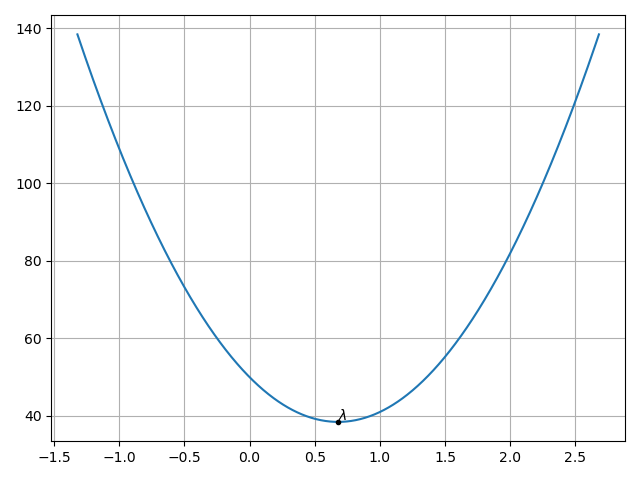
\includegraphics[width=\columnwidth]{11/10/3/14/conv/figs/convex.png}
        \caption{This convex function achieves its minimum at $\lambda_m$.}
        \label{fig:11/10/3/14/conv/convex}
    \end{figure}

			\item  Gradient Descent
				\\
\label{11/10/3/14/grad}
\iffalse
\documentclass[journal,12pt,twocolumn]{IEEEtran}
\usepackage{setspace}
\usepackage{gensymb}
\singlespacing
\usepackage[cmex10]{amsmath}
\usepackage{amsthm}
\usepackage{mathrsfs}
\usepackage{txfonts}
\usepackage{stfloats}
\usepackage{bm}
\usepackage{cite}
\usepackage{cases}
\usepackage{subfig}
\usepackage{longtable}
\usepackage{multirow}
\usepackage{enumitem}
\usepackage{mathtools}
\usepackage{tikz}
\usepackage{circuitikz}
\usepackage{verbatim}
\usepackage[breaklinks=true]{hyperref}
\usepackage{tkz-euclide} % loads  TikZ and tkz-base
\usepackage{listings}
\usepackage{color}    
\usepackage{array}    
\usepackage{longtable}
\usepackage{calc}     
\usepackage{multirow} 
\usepackage{hhline}   
\usepackage{ifthen}   
\usepackage{lscape}     
\usepackage{chngcntr}
\DeclareMathOperator*{\Res}{Res}
\renewcommand\thesection{\arabic{section}}
\renewcommand\thesubsection{\thesection.\arabic{subsection}}
\renewcommand\thesubsubsection{\thesubsection.\arabic{subsubsection}}

\renewcommand\thesectiondis{\arabic{section}}
\renewcommand\thesubsectiondis{\thesectiondis.\arabic{subsection}}
\renewcommand\thesubsubsectiondis{\thesubsectiondis.\arabic{subsubsection}}
\renewcommand\thetable{\arabic{table}}
% correct bad hyphenation here
\hyphenation{op-tical net-works semi-conduc-tor}
\def\inputGnumericTable{}                                 %%

\lstset{
%language=C,
frame=single, 
breaklines=true,
columns=fullflexible
}
%\lstset{
%language=tex,
%frame=single, 
%breaklines=true
%}

\begin{document}
\newtheorem{theorem}{Theorem}[section]
\newtheorem{problem}{Problem}
\newtheorem{proposition}{Proposition}[section]
\newtheorem{lemma}{Lemma}[section]
\newtheorem{corollary}[theorem]{Corollary}
\newtheorem{example}{Example}[section]
\newtheorem{definition}[problem]{Definition}
\newcommand{\BEQA}{\begin{eqnarray}}
\newcommand{\EEQA}{\end{eqnarray}}
\newcommand{\define}{\stackrel{\triangle}{=}}
\bibliographystyle{IEEEtran}
\providecommand{\mbf}{\mathbf}
\providecommand{\pr}[1]{\ensuremath{\Pr\left(#1\right)}}
\providecommand{\qfunc}[1]{\ensuremath{Q\left(#1\right)}}
\providecommand{\sbrak}[1]{\ensuremath{{}\left[#1\right]}}
\providecommand{\lsbrak}[1]{\ensuremath{{}\left[#1\right.}}
\providecommand{\rsbrak}[1]{\ensuremath{{}\left.#1\right]}}
\providecommand{\brak}[1]{\ensuremath{\left(#1\right)}}
\providecommand{\lbrak}[1]{\ensuremath{\left(#1\right.}}
\providecommand{\rbrak}[1]{\ensuremath{\left.#1\right)}}
\providecommand{\cbrak}[1]{\ensuremath{\left\{#1\right\}}}
\providecommand{\lcbrak}[1]{\ensuremath{\left\{#1\right.}}
\providecommand{\rcbrak}[1]{\ensuremath{\left.#1\right\}}}
\theoremstyle{remark}
\newtheorem{rem}{Remark}
\newcommand{\sgn}{\mathop{\mathrm{sgn}}}
\providecommand{\abs}[1]{\left\vert#1\right\vert}
\providecommand{\res}[1]{\Res\displaylimits_{#1}} 
\providecommand{\norm}[1]{\left\lVert#1\right\rVert}
\providecommand{\mtx}[1]{\mathbf{#1}}
\providecommand{\mean}[1]{E\left[ #1 \right]}
\providecommand{\fourier}{\overset{\mathcal{F}}{ \rightleftharpoons}}
\providecommand{\system}[1]{\overset{\mathcal{#1}}{ \longleftrightarrow}}
\newcommand{\solution}{\noindent \textbf{Solution: }}
\newcommand{\cosec}{\,\text{cosec}\,}
\providecommand{\dec}[2]{\ensuremath{\overset{#1}{\underset{#2}{\gtrless}}}}
\newcommand{\myvec}[1]{\ensuremath{\begin{pmatrix}#1\end{pmatrix}}}
\newcommand{\mydet}[1]{\ensuremath{\begin{vmatrix}#1\end{vmatrix}}}
\let\vec\mathbf
\def\putbox#1#2#3{\makebox[0in][l]{\makebox[#1][l]{}\raisebox{\baselineskip}[0in][0in]{\raisebox{#2}[0in][0in]{#3}}}}
     \def\rightbox#1{\makebox[0in][r]{#1}}
     \def\centbox#1{\makebox[0in]{#1}}
     \def\topbox#1{\raisebox{-\baselineskip}[0in][0in]{#1}}
     \def\midbox#1{\raisebox{-0.5\baselineskip}[0in][0in]{#1}}

\vspace{3cm}
\title{Optimization Assignment}
\author{Gautam Singh}
\maketitle
\bigskip

\begin{abstract}
    This document contains the solution to Question 4 of Exercise 2 in Chapter
    10 of the class 11 NCERT textbook.
\end{abstract}

\begin{enumerate}
  
    \solution 
\fi
		Any point on \eqref{eq:11/10/3/14/grad/line} is clearly of the form
    \begin{align}
        \vec{Q} = \vec{A} + \lambda\vec{m}
        \label{eq:11/10/3/14/grad/Q-def}
    \end{align}
    where $\lambda \in \mathbb{R}$ and
    \begin{align}
        \vec{A} = \myvec{0\\-4},\ \vec{m} = \myvec{4\\3}
        \label{eq:11/10/3/14/grad/vals}
    \end{align}
    Thus,
    \begin{align}
        f\brak{\lambda} &= \norm{\vec{Q}-\vec{P}}^2 \\
                        &= \norm{\vec{A}-\vec{P}+\lambda\vec{m}}^2 \\
                        &= \norm{\vec{m}}^2\lambda^2 + 2\vec{m}^\top\brak{\vec{A}-\vec{P}}\lambda + \norm{\vec{A}-\vec{P}}^2
                        \label{eq:11/10/3/14/grad/dist-lambda}
    \end{align}
    Since \eqref{eq:11/10/3/14/grad/dist-lambda} is convex, we use the gradient descent function 
    on $\lambda$ to converge at the minimum of $f\brak{\lambda}$.
    \begin{align}
        \lambda_{n+1} &= \lambda_n - \alpha f'\brak{\lambda_n} \\
                      &= \brak{1-2\alpha\norm{\vec{m}}^2}\lambda_n + 2\alpha\vec{m}^\top\brak{\vec{A}-\vec{P}}
                      \label{eq:11/10/3/14/grad/diff-eqn}
    \end{align}
    Taking the one-sided $Z$-transform on both sides of \eqref{eq:11/10/3/14/grad/diff-eqn},
    \begin{align}
        z\Lambda\brak{z} &= \brak{1-2\alpha\norm{\vec{m}}^2}\Lambda\brak{z} - \frac{2\alpha\vec{m}^\top\brak{\vec{A}-\vec{P}}}{1-z^{-1}}
        \label{eq:11/10/3/14/grad/Z-trans-eqn}
    \end{align}
    Solving \eqref{eq:11/10/3/14/grad/Z-trans-eqn}
    \begin{align}
        &\Lambda\brak{z} = -\frac{2\alpha\vec{m}^\top\brak{\vec{A}-\vec{P}}z^{-1}}{\brak{1- z^{-1}}\brak{1 - \brak{1-2\alpha\norm{\vec{m}}^2}z^{-1}}} \label{eq:11/10/3/14/grad/roc} \\
        &= -\frac{\vec{m}^\top\brak{\vec{A}-\vec{P}}}{\norm{\vec{m}}^2}\lbrak{\frac{1}{1-z^{-1}}} \\
        &\rbrak{- \frac{1}{1-\brak{1-2\alpha\norm{\vec{m}}^2}z^{-1}}} \\
        &= \frac{\vec{m}^\top\brak{\vec{A}-\vec{P}}}{\norm{\vec{m}}^2}\sum_{k=0}^{\infty}\brak{1-\brak{1-2\alpha\norm{\vec{m}}^2}^k}z^{-k}
        \label{eq:11/10/3/14/grad/lambda-z-trans}
    \end{align}
    From \eqref{eq:11/10/3/14/grad/roc}, the ROC is
    \begin{align}
        \abs{z} &> \max\cbrak{1,1-2\alpha\norm{\vec{m}}^2} \\
        \implies 0 &< 1 - 2\alpha\norm{\vec{m}}^2 < 1 \\
        \implies 0 &< \alpha < \frac{1}{2\norm{\vec{m}}^2}
        \label{eq:11/10/3/14/grad/alpha-constr}
    \end{align}
    Thus, if $\alpha$ satisfies \eqref{eq:11/10/3/14/grad/alpha-constr}, then from 
    \eqref{eq:11/10/3/14/grad/lambda-z-trans}, substituting from \eqref{eq:11/10/3/14/grad/vals},
    \begin{align}
        \lim_{n\to\infty}\lambda_n &= -\frac{\vec{m}^\top\brak{\vec{A}-\vec{P}}}{\norm{\vec{m}^2}}                                  \label{eq:11/10/3/14/grad/conv}
                                   &= \frac{17}{25}
    \end{align}
    We select the following parameters to arrive at the optimal $\lambda$,
    where $N$ is the number of iterations and $\epsilon$ is the convergence 
    limit. The gradient descent is demonstrated in Fig. \ref{fig:11/10/3/14/grad/grad-desc},
    plotted by the Python code. The relevant
    parameters are shown in Table \ref{tab:11/10/3/14/grad/param}.
    \begin{table}[!ht]
        \centering
        %%%%%%%%%%%%%%%%%%%%%%%%%%%%%%%%%%%%%%%%%%%%%%%%%%%%%%%%%%%%%%%%%%%%%%
%%                                                                  %%
%%  This is the header of a LaTeX2e file exported from Gnumeric.    %%
%%                                                                  %%
%%  This file can be compiled as it stands or included in another   %%
%%  LaTeX document. The table is based on the longtable package so  %%
%%  the longtable options (headers, footers...) can be set in the   %%
%%  preamble section below (see PRAMBLE).                           %%
%%                                                                  %%
%%  To include the file in another, the following two lines must be %%
%%  in the including file:                                          %%
%%        \def\inputGnumericTable{}                                 %%
%%  at the beginning of the file and:                               %%
%%        \input{name-of-this-file.tex}                             %%
%%  where the table is to be placed. Note also that the including   %%
%%  file must use the following packages for the table to be        %%
%%  rendered correctly:                                             %%
%%    \usepackage[latin1]{inputenc}                                 %%
%%    \usepackage{color}                                            %%
%%    \usepackage{array}                                            %%
%%    \usepackage{longtable}                                        %%
%%    \usepackage{calc}                                             %%
%%    \usepackage{multirow}                                         %%
%%    \usepackage{hhline}                                           %%
%%    \usepackage{ifthen}                                           %%
%%  optionally (for landscape tables embedded in another document): %%
%%    \usepackage{lscape}                                           %%
%%                                                                  %%
%%%%%%%%%%%%%%%%%%%%%%%%%%%%%%%%%%%%%%%%%%%%%%%%%%%%%%%%%%%%%%%%%%%%%%



%%  This section checks if we are begin input into another file or  %%
%%  the file will be compiled alone. First use a macro taken from   %%
%%  the TeXbook ex 7.7 (suggestion of Han-Wen Nienhuys).            %%
\def\ifundefined#1{\expandafter\ifx\csname#1\endcsname\relax}


%%  Check for the \def token for inputed files. If it is not        %%
%%  defined, the file will be processed as a standalone and the     %%
%%  preamble will be used.                                          %%
\ifundefined{inputGnumericTable}

%%  We must be able to close or not the document at the end.        %%
	\def\gnumericTableEnd{\end{document}}


%%%%%%%%%%%%%%%%%%%%%%%%%%%%%%%%%%%%%%%%%%%%%%%%%%%%%%%%%%%%%%%%%%%%%%
%%                                                                  %%
%%  This is the PREAMBLE. Change these values to get the right      %%
%%  paper size and other niceties.                                  %%
%%                                                                  %%
%%%%%%%%%%%%%%%%%%%%%%%%%%%%%%%%%%%%%%%%%%%%%%%%%%%%%%%%%%%%%%%%%%%%%%

	\documentclass[12pt%
			  %,landscape%
                    ]{report}
       \usepackage[latin1]{inputenc}
       \usepackage{fullpage}
       \usepackage{color}
       \usepackage{array}
       \usepackage{longtable}
       \usepackage{calc}
       \usepackage{multirow}
       \usepackage{hhline}
       \usepackage{ifthen}

	\begin{document}


%%  End of the preamble for the standalone. The next section is for %%
%%  documents which are included into other LaTeX2e files.          %%
\else

%%  We are not a stand alone document. For a regular table, we will %%
%%  have no preamble and only define the closing to mean nothing.   %%
    \def\gnumericTableEnd{}

%%  If we want landscape mode in an embedded document, comment out  %%
%%  the line above and uncomment the two below. The table will      %%
%%  begin on a new page and run in landscape mode.                  %%
%       \def\gnumericTableEnd{\end{landscape}}
%       \begin{landscape}


%%  End of the else clause for this file being \input.              %%
\fi

%%%%%%%%%%%%%%%%%%%%%%%%%%%%%%%%%%%%%%%%%%%%%%%%%%%%%%%%%%%%%%%%%%%%%%
%%                                                                  %%
%%  The rest is the gnumeric table, except for the closing          %%
%%  statement. Changes below will alter the table's appearance.     %%
%%                                                                  %%
%%%%%%%%%%%%%%%%%%%%%%%%%%%%%%%%%%%%%%%%%%%%%%%%%%%%%%%%%%%%%%%%%%%%%%

\providecommand{\gnumericmathit}[1]{#1} 
%%  Uncomment the next line if you would like your numbers to be in %%
%%  italics if they are italizised in the gnumeric table.           %%
%\renewcommand{\gnumericmathit}[1]{\mathit{#1}}
\providecommand{\gnumericPB}[1]%
{\let\gnumericTemp=\\#1\let\\=\gnumericTemp\hspace{0pt}}
 \ifundefined{gnumericTableWidthDefined}
        \newlength{\gnumericTableWidth}
        \newlength{\gnumericTableWidthComplete}
        \newlength{\gnumericMultiRowLength}
        \global\def\gnumericTableWidthDefined{}
 \fi
%% The following setting protects this code from babel shorthands.  %%
 \ifthenelse{\isundefined{\languageshorthands}}{}{\languageshorthands{english}}
%%  The default table format retains the relative column widths of  %%
%%  gnumeric. They can easily be changed to c, r or l. In that case %%
%%  you may want to comment out the next line and uncomment the one %%
%%  thereafter                                                      %%
\providecommand\gnumbox{\makebox[0pt]}
%%\providecommand\gnumbox[1][]{\makebox}

%% to adjust positions in multirow situations                       %%
\setlength{\bigstrutjot}{\jot}
\setlength{\extrarowheight}{\doublerulesep}

%%  The \setlongtables command keeps column widths the same across  %%
%%  pages. Simply comment out next line for varying column widths.  %%
\setlongtables

\setlength\gnumericTableWidth{%
	62pt+%
	67pt+%
0pt}
\def\gumericNumCols{2}
\setlength\gnumericTableWidthComplete{\gnumericTableWidth+%
         \tabcolsep*\gumericNumCols*2+\arrayrulewidth*\gumericNumCols}
\ifthenelse{\lengthtest{\gnumericTableWidthComplete > \linewidth}}%
         {\def\gnumericScale{1*\ratio{\linewidth-%
                        \tabcolsep*\gumericNumCols*2-%
                        \arrayrulewidth*\gumericNumCols}%
{\gnumericTableWidth}}}%
{\def\gnumericScale{1}}

%%%%%%%%%%%%%%%%%%%%%%%%%%%%%%%%%%%%%%%%%%%%%%%%%%%%%%%%%%%%%%%%%%%%%%
%%                                                                  %%
%% The following are the widths of the various columns. We are      %%
%% defining them here because then they are easier to change.       %%
%% Depending on the cell formats we may use them more than once.    %%
%%                                                                  %%
%%%%%%%%%%%%%%%%%%%%%%%%%%%%%%%%%%%%%%%%%%%%%%%%%%%%%%%%%%%%%%%%%%%%%%

\ifthenelse{\isundefined{\gnumericColA}}{\newlength{\gnumericColA}}{}\settowidth{\gnumericColA}{\begin{tabular}{@{}p{62pt*\gnumericScale}@{}}x\end{tabular}}
\ifthenelse{\isundefined{\gnumericColB}}{\newlength{\gnumericColB}}{}\settowidth{\gnumericColB}{\begin{tabular}{@{}p{67pt*\gnumericScale}@{}}x\end{tabular}}

\begin{tabular}[c]{%
	b{\gnumericColA}%
	b{\gnumericColB}%
	}

%%%%%%%%%%%%%%%%%%%%%%%%%%%%%%%%%%%%%%%%%%%%%%%%%%%%%%%%%%%%%%%%%%%%%%
%%  The longtable options. (Caption, headers... see Goosens, p.124) %%
%	\caption{The Table Caption.}             \\	%
% \hline	% Across the top of the table.
%%  The rest of these options are table rows which are placed on    %%
%%  the first, last or every page. Use \multicolumn if you want.    %%

%%  Header for the first page.                                      %%
%	\multicolumn{2}{c}{The First Header} \\ \hline 
%	\multicolumn{1}{c}{colTag}	%Column 1
%	&\multicolumn{1}{c}{colTag}	\\ \hline %Last column
%	\endfirsthead

%%  The running header definition.                                  %%
%	\hline
%	\multicolumn{2}{l}{\ldots\small\slshape continued} \\ \hline
%	\multicolumn{1}{c}{colTag}	%Column 1
%	&\multicolumn{1}{c}{colTag}	\\ \hline %Last column
%	\endhead

%%  The running footer definition.                                  %%
%	\hline
%	\multicolumn{2}{r}{\small\slshape continued\ldots} \\
%	\endfoot

%%  The ending footer definition.                                   %%
%	\multicolumn{2}{c}{That's all folks} \\ \hline 
%	\endlastfoot
%%%%%%%%%%%%%%%%%%%%%%%%%%%%%%%%%%%%%%%%%%%%%%%%%%%%%%%%%%%%%%%%%%%%%%

\hhline{|-|-}
	 \multicolumn{1}{|p{\gnumericColA}|}%
	{\gnumericPB{\centering}\gnumbox{\textbf{Parameter}}}
	&\multicolumn{1}{p{\gnumericColB}|}%
	{\gnumericPB{\centering}\gnumbox{\textbf{Value}}}
\\
\hhline{|--|}
	 \multicolumn{1}{|p{\gnumericColA}|}%
	{\gnumericPB{\centering}\gnumbox{$\lambda_0$}}
	&\multicolumn{1}{p{\gnumericColB}|}%
	{\gnumericPB{\centering}\gnumbox{0}}
\\
\hhline{|--|}
	 \multicolumn{1}{|p{\gnumericColA}|}%
	{\gnumericPB{\centering}\gnumbox{$\alpha$}}
	&\multicolumn{1}{p{\gnumericColB}|}%
    {\gnumericPB{\centering}\gnumbox{$0.1$}}
\\
\hhline{|--|}
	 \multicolumn{1}{|p{\gnumericColA}|}%
	{\gnumericPB{\centering}\gnumbox{$N$}}
	&\multicolumn{1}{p{\gnumericColB}|}%
    {\gnumericPB{\centering}\gnumbox{$1000000$}}
\\
\hhline{|--|}
	 \multicolumn{1}{|p{\gnumericColA}|}%
	{\gnumericPB{\centering}\gnumbox{$\epsilon$}}
	&\multicolumn{1}{p{\gnumericColB}|}%
    {\gnumericPB{\centering}\gnumbox{$10^{-6}$}}
\\
\hhline{|-|-|}
\end{tabular}

\ifthenelse{\isundefined{\languageshorthands}}{}{\languageshorthands{\languagename}}
\gnumericTableEnd

        \caption{Parameters for Gradient Descent}
        \label{tab:11/10/3/14/grad/param}
    \end{table}

    \begin{figure}[!ht]
        \centering
        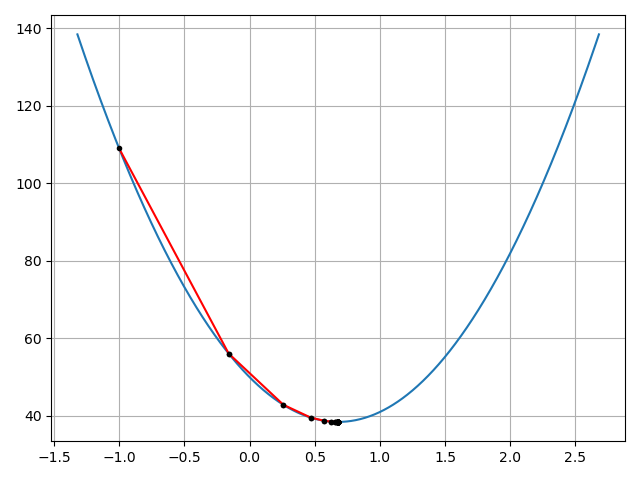
\includegraphics[width=\columnwidth]{11/10/3/14/grad/figs/grad_desc.png}
        \caption{Gradient descent to get the optimal $\lambda$.}
        \label{fig:11/10/3/14/grad/grad-desc}
    \end{figure}

%
\item  Lagrange Multipliers
\\
\solution 
\label{11/10/3/14/lagmul}
\iffalse
\documentclass[journal,12pt,twocolumn]{IEEEtran}
\usepackage{setspace}
\usepackage{gensymb}
\singlespacing
\usepackage[cmex10]{amsmath}
\usepackage{amsthm}
\usepackage{mathrsfs}
\usepackage{txfonts}
\usepackage{stfloats}
\usepackage{bm}
\usepackage{cite}
\usepackage{cases}
\usepackage{subfig}
\usepackage{longtable}
\usepackage{multirow}
\usepackage{enumitem}
\usepackage{mathtools}
\usepackage{tikz}
\usepackage{circuitikz}
\usepackage{verbatim}
\usepackage[breaklinks=true]{hyperref}
\usepackage{tkz-euclide} % loads  TikZ and tkz-base
\usepackage{listings}
\usepackage{color}    
\usepackage{array}    
\usepackage{longtable}
\usepackage{calc}     
\usepackage{multirow} 
\usepackage{hhline}   
\usepackage{ifthen}   
\usepackage{lscape}     
\usepackage{chngcntr}
\DeclareMathOperator*{\Res}{Res}
\renewcommand\thesection{\arabic{section}}
\renewcommand\thesubsection{\thesection.\arabic{subsection}}
\renewcommand\thesubsubsection{\thesubsection.\arabic{subsubsection}}

\renewcommand\thesectiondis{\arabic{section}}
\renewcommand\thesubsectiondis{\thesectiondis.\arabic{subsection}}
\renewcommand\thesubsubsectiondis{\thesubsectiondis.\arabic{subsubsection}}
\renewcommand\thetable{\arabic{table}}
% correct bad hyphenation here
\hyphenation{op-tical net-works semi-conduc-tor}
\def\inputGnumericTable{}                                 %%

\lstset{
%language=C,
frame=single, 
breaklines=true,
columns=fullflexible
}
%\lstset{
%language=tex,
%frame=single, 
%breaklines=true
%}

\begin{document}
\newtheorem{theorem}{Theorem}[section]
\newtheorem{problem}{Problem}
\newtheorem{proposition}{Proposition}[section]
\newtheorem{lemma}{Lemma}[section]
\newtheorem{corollary}[theorem]{Corollary}
\newtheorem{example}{Example}[section]
\newtheorem{definition}[problem]{Definition}
\newcommand{\BEQA}{\begin{eqnarray}}
\newcommand{\EEQA}{\end{eqnarray}}
\newcommand{\define}{\stackrel{\triangle}{=}}
\bibliographystyle{IEEEtran}
\providecommand{\mbf}{\mathbf}
\providecommand{\pr}[1]{\ensuremath{\Pr\left(#1\right)}}
\providecommand{\qfunc}[1]{\ensuremath{Q\left(#1\right)}}
\providecommand{\sbrak}[1]{\ensuremath{{}\left[#1\right]}}
\providecommand{\lsbrak}[1]{\ensuremath{{}\left[#1\right.}}
\providecommand{\rsbrak}[1]{\ensuremath{{}\left.#1\right]}}
\providecommand{\brak}[1]{\ensuremath{\left(#1\right)}}
\providecommand{\lbrak}[1]{\ensuremath{\left(#1\right.}}
\providecommand{\rbrak}[1]{\ensuremath{\left.#1\right)}}
\providecommand{\cbrak}[1]{\ensuremath{\left\{#1\right\}}}
\providecommand{\lcbrak}[1]{\ensuremath{\left\{#1\right.}}
\providecommand{\rcbrak}[1]{\ensuremath{\left.#1\right\}}}
\theoremstyle{remark}
\newtheorem{rem}{Remark}
\newcommand{\sgn}{\mathop{\mathrm{sgn}}}
\providecommand{\abs}[1]{\left\vert#1\right\vert}
\providecommand{\res}[1]{\Res\displaylimits_{#1}} 
\providecommand{\norm}[1]{\left\lVert#1\right\rVert}
\providecommand{\mtx}[1]{\mathbf{#1}}
\providecommand{\mean}[1]{E\left[ #1 \right]}
\providecommand{\fourier}{\overset{\mathcal{F}}{ \rightleftharpoons}}
\providecommand{\system}[1]{\overset{\mathcal{#1}}{ \longleftrightarrow}}
\newcommand{\solution}{\noindent \textbf{Solution: }}
\newcommand{\cosec}{\,\text{cosec}\,}
\providecommand{\dec}[2]{\ensuremath{\overset{#1}{\underset{#2}{\gtrless}}}}
\newcommand{\myvec}[1]{\ensuremath{\begin{pmatrix}#1\end{pmatrix}}}
\newcommand{\mydet}[1]{\ensuremath{\begin{vmatrix}#1\end{vmatrix}}}
\let\vec\mathbf
\def\putbox#1#2#3{\makebox[0in][l]{\makebox[#1][l]{}\raisebox{\baselineskip}[0in][0in]{\raisebox{#2}[0in][0in]{#3}}}}
     \def\rightbox#1{\makebox[0in][r]{#1}}
     \def\centbox#1{\makebox[0in]{#1}}
     \def\topbox#1{\raisebox{-\baselineskip}[0in][0in]{#1}}
     \def\midbox#1{\raisebox{-0.5\baselineskip}[0in][0in]{#1}}

\vspace{3cm}
\title{Optimization Assignment}
\author{Gautam Singh}
\maketitle
\bigskip

\begin{abstract}
    This document contains the solution to Question 4 of Exercise 2 in Chapter
    10 of the class 11 NCERT textbook.
\end{abstract}

\begin{enumerate}
  
    \solution 
    \fi
		We rewrite the problem as
    \begin{align}
        \min_{\vec{x}} h\brak{\vec{x}} &\triangleq \norm{\vec{x}-\vec{P}}^2 \\
        \textrm{s.t. } g\brak{\vec{x}} &\triangleq \vec{n}^\top\vec{x} - c = 0
        \label{eq:11/10/3/14/lagmul/lag-opt}
    \end{align}
    where
    \begin{align}
        \vec{P} = \myvec{-1\\3},\ \vec{n} = \myvec{3\\-4},\ c = 16
        \label{eq:11/10/3/14/lagmul/vals}
    \end{align}
    Define
    \begin{align}
        C\brak{\vec{x},\lambda} &= h\brak{\vec{x}} - \lambda g\brak{\vec{x}}
        \label{eq:11/10/3/14/lagmul/C-def}
    \end{align}
    and note that
    \begin{align}
        \nabla h\brak{\vec{x}} &= 2\brak{\vec{x}-\vec{P}} \\
        \nabla g\brak{\vec{x}} &= \vec{n}
        \label{eq:11/10/3/14/lagmul/diff-gh}
    \end{align}
    We are required to find $\lambda \in \mathbb{R}$ such that
    \begin{align}
        \nabla C\brak{\vec{x},\lambda} &= 0 \\
        \implies 2\brak{\vec{x}-\vec{P}} - \lambda\vec{n} &= 0
        \label{eq:11/10/3/14/lagmul/x-lambda}
    \end{align}
    However, $\vec{x}$ lies on the line \eqref{eq:11/10/3/14/lagmul/line}. Thus, from
    \eqref{eq:11/10/3/14/lagmul/x-lambda},
    \begin{align}
        \vec{n}^\top\brak{\frac{\lambda}{2}\vec{n}+\vec{P}} - c &= 0 \\
        \implies \lambda &= \frac{2\brak{c-\vec{n}^\top\vec{P}}}{\norm{\vec{n}}^2}
        \label{eq:11/10/3/14/lagmul/lambda-opt}
    \end{align}
    Substituting \eqref{eq:11/10/3/14/lagmul/lambda-opt} in \eqref{eq:11/10/3/14/lagmul/x-lambda}, the optimal
    point is given by
    \begin{align}
        \vec{Q} &= \vec{P} + \frac{\lambda}{2}\vec{n} \\
                &= \vec{P} - \frac{\vec{n}^\top\vec{P}-c}{\norm{\vec{n}}^2}\vec{n}
                \label{eq:11/10/3/14/lagmul/x-sol-lag}
    \end{align}
    Substituting from \eqref{eq:11/10/3/14/lagmul/vals},
    \begin{align}
        \lambda = \frac{62}{25},\ \vec{Q} = \frac{1}{25}\myvec{68\\-49}
        \label{eq:11/10/3/14/lagmul/sol}
    \end{align}
    To find $\vec{Q}$ graphically, we use constrained gradient descent, with
    learning rate $\alpha = 0.01$. The results are shown in Fig.
    \ref{fig:11/10/3/14/lagmul/gd-lag}, plotted using the Python code.
    \begin{figure}[!ht]
        \centering
        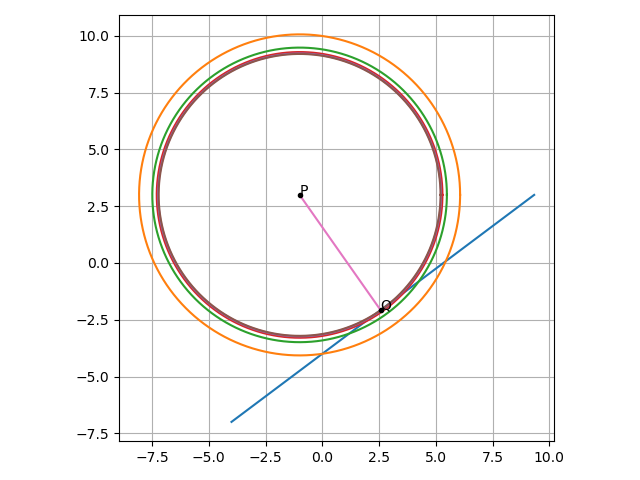
\includegraphics[width=\columnwidth]{11/10/3/14/lagmul/figs/gd_lagrange.png}
        \caption{Constrained gradient descent to find optimal $\vec{Q}$.}
        \label{fig:11/10/3/14/lagmul/gd-lag}
    \end{figure}
\textit{Constrained gradient descent} is a method of optimizing the cost function
subject to some constraints, represented as follows.
\begin{align}
    \max_{\vec{x}}f\brak{\vec{x}} \label{eq:11/10/3/14/lagmul/cgd-cost} \\
    \textrm{s.t. } g\brak{\vec{x}} = 0
    \label{eq:11/10/3/14/lagmul/cgd-constr}
\end{align}
Unlike the unconstrained version, one cannot move in the negative direction of the
gradient vector of $f\brak{\vec{x}}$. However, we must move along the constraint in
\eqref{eq:11/10/3/14/lagmul/cgd-constr}.

The algorithm terminates when the gradient vector of $f$ is parallel to the normal 
vector of $g$ at that point. Mathematically, at an optimum $\vec{x_o}$,
\begin{align}
    \nabla f\brak{\vec{x_o}} = \lambda\nabla g\brak{\vec{x_o}}
    \label{eq:11/10/3/14/lagmul/cgd-cond}
\end{align}
where $\lambda \in \mathbb{R}\setminus\cbrak{0}$. Observe that \eqref{eq:11/10/3/14/lagmul/cgd-cond}
may be rewritten as
\begin{align}
    \nabla C\brak{\vec{x},\lambda} = \nabla \brak{f\brak{\vec{x}}-\lambda g\brak{\vec{x}}} = 0
\end{align}
which is analogous to the method of Lagrangian multipliers.

		\end{enumerate}


\end{enumerate}
